
\documentclass{article}
\usepackage{graphicx}
\usepackage{float}

\begin{document}
\title{Classification of activities on Netgear router}
\author{Abhinav Narain}
\maketitle

\section{Benchmarks}
We want micro benchmarks to suggest how good or bad the technique
we are using. These benchmarks will vary depending on the device if we
want to do activity recognition (for example,camera might run
different applications than a photo-frame.) but might remain the same
for basic activities done by malware.

As suggested by Kyle, I have simulated malware activities, instead of
running actual malware. 

I have done classification for the following activities with the
technique and the results in the section~\ref{sec:technique} and
section~\ref{sec:results}
\begin{itemize}
\item DNS packet flood attack
\item UDP flood attack with payload of 1460 bytes
\item UDP flood attack with payload of 730 bytes
\item Router with default firmware running (Idle)
\item Computation
\end{itemize}

There are set of benchmarks I wanted to do but was unable to proceed
and reasons that it was not possible.
\begin{itemize}
\item Experiments with measurements of L1, L2, L3 caches
  \begin{itemize}
  \item Router does not have many levels of caches as dmesg shows~\ref{subsec:dmesg}
  \end{itemize}
\item copying a file (using Linux command \textit{dd})
  \begin{itemize}
  \item Does not have enough memory to copy files for recording it
  \end{itemize}
\end{itemize}

Figure~\ref{fig:wireless} shows the change in EMI due to turning
hardware switch on or off for the router~\ref{fig:router}. This is
significant change due turning on/off the wireless subsystem which
wasn't present in case of laptop. There is clearly a wide difference
in the proportion of power consumption among the subsystems.

\section{Technique}\label{sec:technique}
Although there is large EMI that is produced by the
The difference between Discret Wavelet Transform (DWT) and Wavelet
Packet Decomposition (WPT), WPT decomposes the signal space into a
huge binary tree, while DWT only decomposes the left branch
recursively.

While decomposition at every level, each of the algorithms (DWT and
WPT) subsample while passing through the Low Pass Filter and High Pass
Filter, succesively reducing the size (by half) of the coefficients
and also partitioning the frequency content as shown in
figure~\ref{fig:explain}.

Sample rate used is 500 KHz and the interesting frequecies are in
80-120KHz range, and hence I have selected the DWT coefficients of the
second node of the first row, which has the range of 128KHz - 256 KHz.

The EMI trace is segmented period of 10ms as shown in Fig~\ref{pulse}.

\subsection{Expected Output of EMI}

\section{Comments}
\begin{enumerate}
\item The results are dependent on the hardware. Raspberry Pi did not
  show any activity using our hardware, while the Netgear Router shows
  significant EMI variation
\item EMI is not very effective in detecting stealthy malware. A
  malware can \textit{sleep} for random time period (for example in
  \textit{mirai} to evade signature detection
\item This is not an end all solution, highly depending on the
  hardware
\item I have also pursued finding if we could use some bulbs etc. to
  do a distributed attack from bunch of IoT devices together
\end{enumerate}
\section{Results}\label{sec:results}
end result
\section{Supplemtary}
\subsection{Spectrograms of the traces}
\begin{figure}[H]
\centering
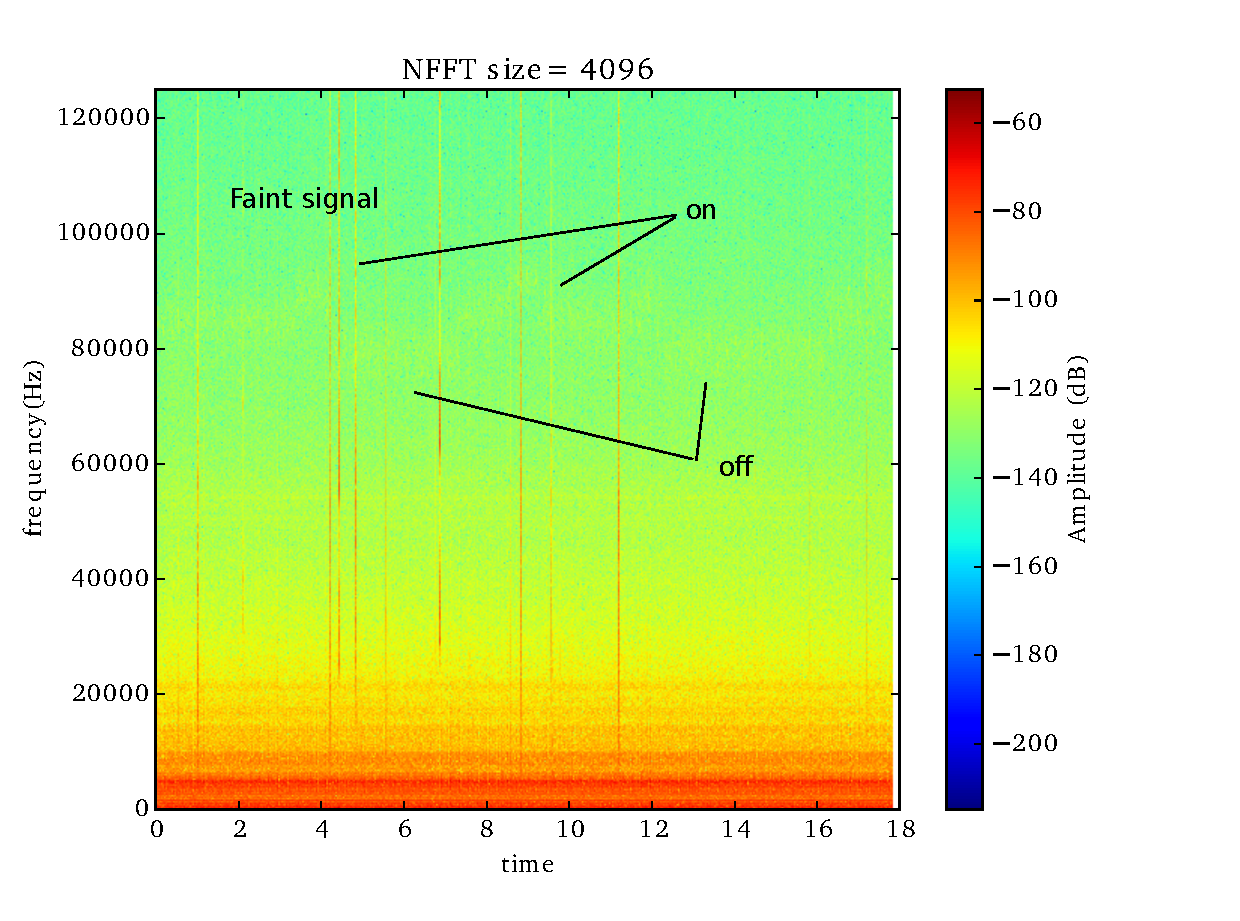
\includegraphics[width=\textwidth]{figures/ww.pdf}
\caption{EMI trace of power-line when the switch powers the wireless
  subsystem on and off. Fs=500kHz}
\label{fig:wireless}
\end{figure}

\begin{figure}[H]
\centering
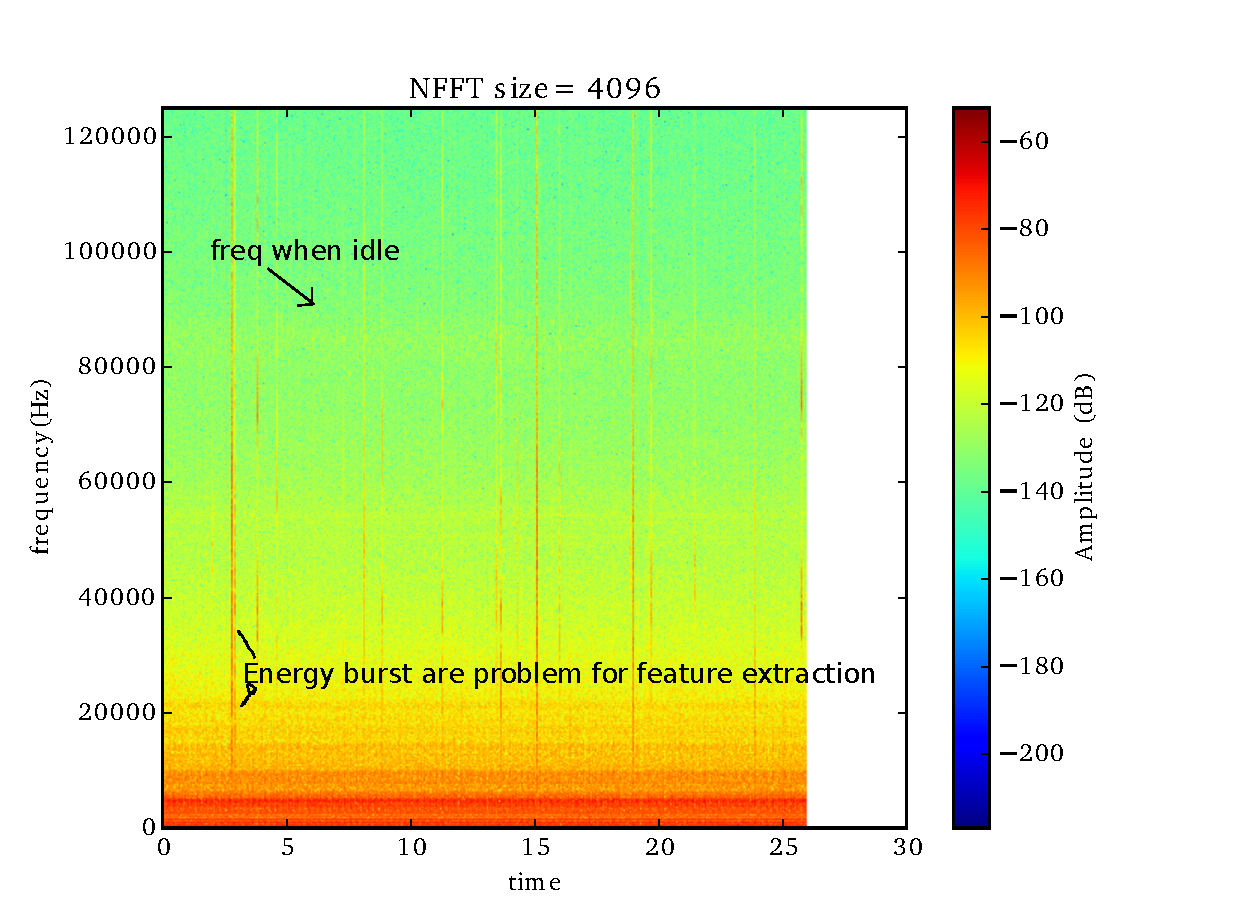
\includegraphics[width=\textwidth]{figures/ii.pdf}
\caption{EMI trace when the router is idle, which means, it is
  not executing any special application/binary installed on it. EMI is
  at ~80KHz. This might be a harmonic for a lower frequency, but it is most
  clear to us and hence indicated in the spectrogram.}
\label{fig:idle}
\end{figure}

\begin{figure}[H]
\centering
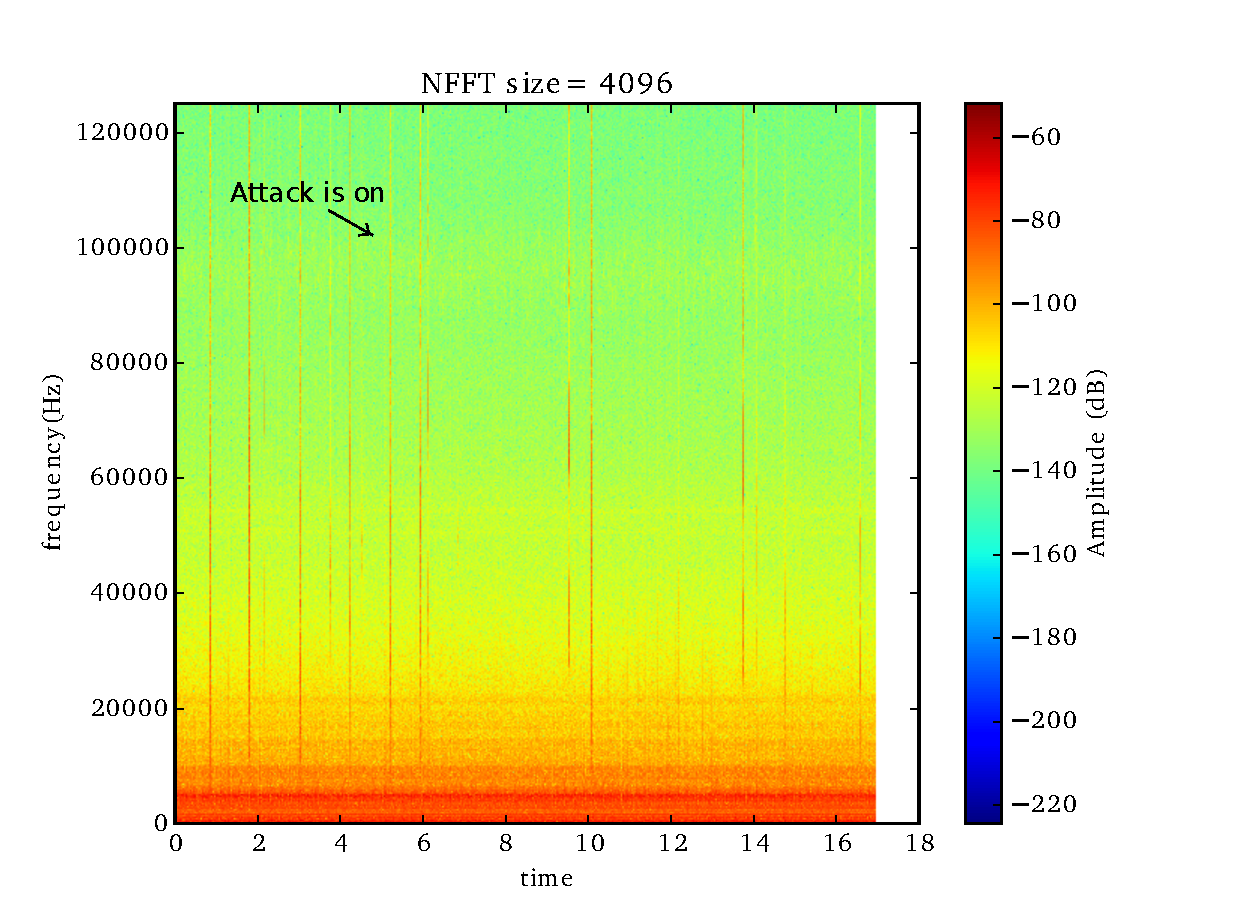
\includegraphics[width=\textwidth]{figures/dd.pdf}
\caption{EMI trace when the router is doing DNS flood attack. The frequency
changes to 100KHz. The same behavior happens when we do UDP flood attack.}
\label{fig:dns}
\end{figure}


\subsection{Time traces of the samples}
\begin{figure}[H]
\centering
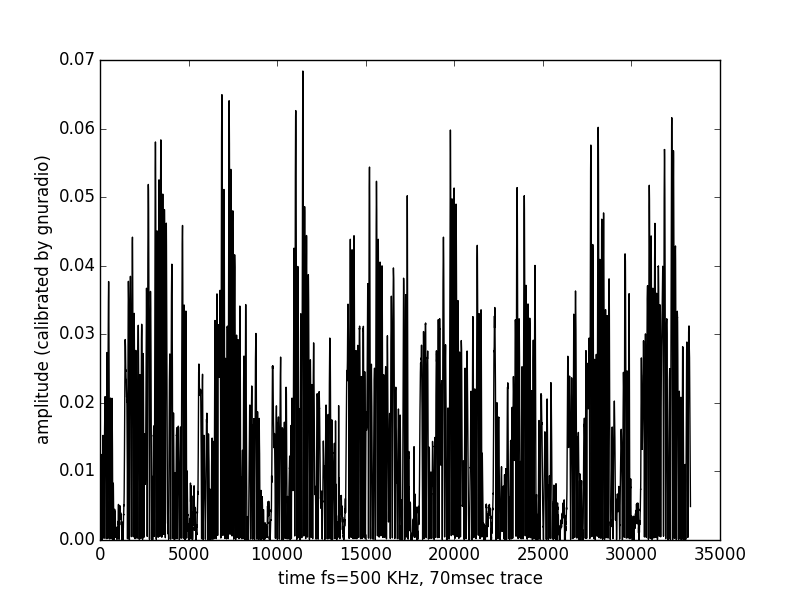
\includegraphics[width=\textwidth]{figures/pulse_train.png}
\caption{Signal trace of router EMI in time domain. This corresponds
  to the alternating bands (cyclo-stationary) of red in spectrogram}
\label{fig:pulse_train}
\end{figure}

\begin{figure}[H]
\centering
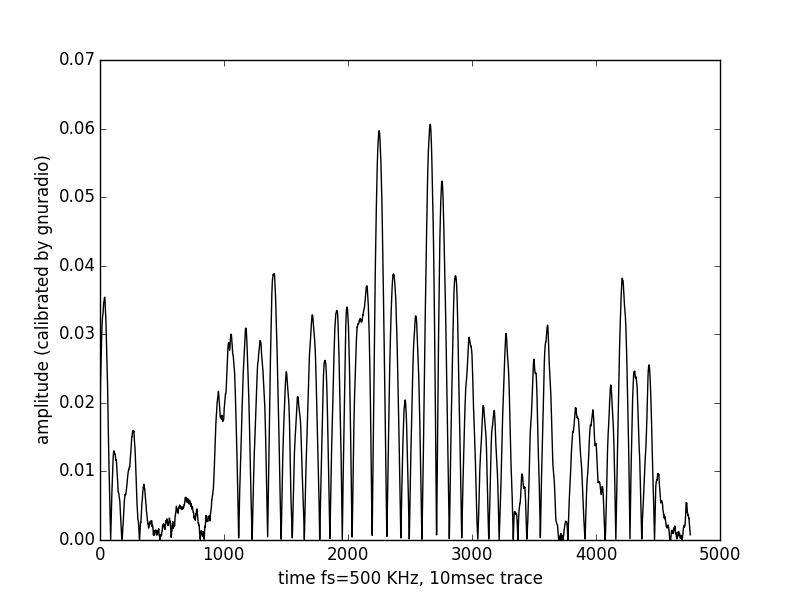
\includegraphics[width=\textwidth]{figures/pulse.png}
\caption{Signal trace of a single segment of router EMI, corresponding
  to one power cycle of the router. This segmented trace is given as a
  feature vector to the classifier}
\label{fig:pulse}
\end{figure}


\subsection{dmesg output}\label{subsec:dmesg}
\textit{dmesg} output suggesting only L1 cache on
router. \textit{lscpu} command was not found even after going through
whole of menconfig/defconfig files while building \textit{OpenWrt}.

\begin{verbatim}
Cached:             6284 kB 
[    0.000000] Primary instruction cache 64kB, VIPT, 4-way, linesize 32 bytes
[    0.000000] Primary data cache 32kB, 4-way, VIPT, cache aliases, linesize 32 bytes
[    0.000000] Dentry cache hash table entries: 16384 (order: 4, 65536 bytes)
[    0.000000] Inode-cache hash table entries: 8192 (order: 3, 32768 bytes)
[    0.086171] Mount-cache hash table entries: 1024 (order: 0, 4096 bytes)
[    0.093221] Mountpoint-cache hash table entries: 1024 (order: 0, 4096 bytes)
\end{verbatim}

\end{document}
